\documentclass{beamer}
\setbeamertemplate{navigation symbols}{}
\setbeamersize{text margin left=0cm, text margin right=0cm}
\usepackage{tcolorbox}
    \tcbuselibrary{skins}
\usepackage{ocgx}
\usepackage{hyperref}

\newtcolorbox{InnerSubjectBox}{
    enhanced,
    nobeforeafter,
    arc=0pt,
    width=.25\paperwidth,
    %height=0.1\paperheight,
    boxrule=1pt,
    colframe=white,
    center upper,
    interior style={
        top color=blue,
        bottom color=black
    },
    valign=center,
    colupper=white,
}

\newcommand{\subjects}[4]{
    \begin{InnerSubjectBox}
        #1
    \end{InnerSubjectBox}%
    \begin{InnerSubjectBox}
        #2
    \end{InnerSubjectBox}%
    \begin{InnerSubjectBox}
        #3
    \end{InnerSubjectBox}%
    \begin{InnerSubjectBox}
        #4
    \end{InnerSubjectBox}
}

\newtcolorbox{InnerPrizeBox}{
    enhanced,
    nobeforeafter,
    arc=0pt,
    width=.25\paperwidth,
    boxrule=.4pt,
    colframe=white,
    center upper,
    interior style={
        top color=blue,
        bottom color=black
    },
    colupper=white,
    valign=center,
    fontupper=\LARGE\bfseries,
    height=.176\paperheight
}

\newcommand{\prizes}{%
    \foreach \i in {1,2,...,4}{%
        \begin{InnerPrizeBox}%
            \begin{ocg}{s\i-100}{s\i-100}{1}{\hyperlink{s\i-100}{100}}\end{ocg}
        \end{InnerPrizeBox}%
        }%

    \foreach \i in {1,2,...,4}{%
        \begin{InnerPrizeBox}%
            \begin{ocg}{s\i-200}{s\i-200}{1}{\hyperlink{s\i-200}{200}}\end{ocg}
        \end{InnerPrizeBox}%
        }%

    \foreach \i in {1,2,...,4}{%
        \begin{InnerPrizeBox}%
            \begin{ocg}{s\i-300}{s\i-300}{1}{\hyperlink{s\i-300}{300}}\end{ocg}
        \end{InnerPrizeBox}%
        }%

    \foreach \i in {1,2,...,4}{%
        \begin{InnerPrizeBox}%
            \begin{ocg}{s\i-400}{s\i-400}{1}{\hyperlink{s\i-400}{400}}\end{ocg}
        \end{InnerPrizeBox}%
        }%

    \foreach \i in {1,2,...,4}{%
        \begin{InnerPrizeBox}%
            \begin{ocg}{s\i-500}{s\i-500}{1}{\hyperlink{s\i-500}{500}}\end{ocg}
        \end{InnerPrizeBox}%
        }%
    }

\newtcolorbox{QuestionHeadFoot}[1][]{
    enhanced,
    before=\vskip-.7ex,
    after=,
    arc=0pt,
    width=\paperwidth,
    boxrule=.4pt,
    colframe=white,
    center upper,
    center lower,
    interior style={
        top color=blue,
        bottom color=black
    },
    colupper=white,
    collower=white,
    valign=center,
    fontupper=\LARGE\bfseries,
    fontlower=\LARGE\bfseries,
    height=.176\paperheight,
    sidebyside,
    segmentation style={white,solid,line width=.4pt},
    #1
}

\newcommand{\header}[2]{
    \begin{QuestionHeadFoot}
        Subject #1 \tcblower #2
    \end{QuestionHeadFoot}
}

\newcommand{\footer}[1]{
    \begin{QuestionHeadFoot}[before=\vskip-2.7ex]
        \hyperlink{question#1}{Question} \\ \hyperlink{answer#1}{Answer} \tcblower
        \hideocg{#1}{Done!} \\ \hyperlink{home}{Home}
    \end{QuestionHeadFoot}
}

\newcommand{\content}[4]{
\begin{frame}
    \hypertarget<1>{question#1}{}
    \hypertarget<2>{answer#1}{}
    \hypertarget{#1}{}
    \header{#2}{#3}
  #4
    \footer{#1}
\end{frame}
}

\newtcolorbox{textarea}[1][]{
    nobeforeafter,
    height=6.2cm,
    boxrule=0pt,
    center upper,
    valign=center,
    #1
}

\begin{document}
\begin{frame}
\hypertarget{home}{}
\vspace*{-.5cm}
    \subjects{DP}{Flow}{Greedy}{Approximation}
    \prizes
\end{frame}

\content                       % 4 arguments
	{s1-100}                     % question internal identifier
	{1}                          % subject number
	{100}{                       % question prize
        \begin{textarea}[]         % question/answer content
        \only<1>{                  % answer content
            What are the steps you use to solve a dynamic programming problem? 
        }
        \only<2>{                  % question content
		Describe recursive structure, define array, state subproblems in array, write iterative code, and if needed, retrace the code to find answer (ex path). Steps do not need to be exactly in this order, or exactly these, but this is the overall process.\\ (\url{https://mcs.utm.utoronto.ca/~zingarod/373/lecture4/lecture4.pdf})
	}
        \end{textarea}
}

\content
	{s1-200}
	{2}
	{200}{
	\begin{textarea}[]
	\only<1>{
		Write out the code for returning an array of the first n Fibonacci numbers. 
	}
	\only<2>{
	def fib(n): \newline
		lst = [0,1] \newline
            	for i in (2...n-1):\newline 
                	lst[i] = lst[i-1] + lst[i-1]\newline 
         return lst
	}
	\end{textarea}
}
\content
	{s1-300}
	{3}
	{300}{
	\begin{textarea}[]
	\only<1>{
Robot Knapsack:
Suppose a robot has capacity of I, and wants to maximise the value of it’s loot. It is located on a checkerboard. The robot can move one of three ways, and must pick up the loot from the position it moves to:
- Up and to the right
- Up and to the left
- Directly upwards.
State the basic recurrence and dimensions for the DP array that would solve this problem.	
	}
	\only<2>{
		We create $m+2 * n+2$ array, DP: \newline 
		DP[i][j] = -inf/0/etc  if i = 0, or if j = 0, or if i=m+1 or j = n+1 (fill in a "border" square around the checkerboard)  \newline
		DP[i][j] =  max{DP[i+1][j+1], DP[i+1][j-1], DP[i][j]} + $v_{i,j}$ where $i <= m$ and $j <= n$ \newline
	}
	\end{textarea}
}
\content
	{s1-400}
	{4}
	{400}{
	\begin{textarea}[]
	\only<1>{
		The Longest Increasing Subsequence (LIS) problem is to find the length of the longest subsequence of a given sequence such that all elements of the subsequence are sorted in increasing order. \newline
		Input  : arr[] = {3, 10, 2, 1, 20} \newline
		Output : Length of LIS = 3 \newline
		The longest increasing subsequence is 3, 10, 20 \newline
	}
	\only<2>{
		Let arr[0..n-1] be the input array and L(i) be the length of the LIS ending at index i such that arr[i] is the last element of the LIS : \newline
L(i) = 1 + max( L(j) ) where 0 < j < i and arr[j] < arr[i]; or \newline
L(i) = 1, if no such j exists.
	}
	\end{textarea}
}
\content
	{s1-500}
	{5}
	{500}{
	\begin{textarea}[]
	\only<1>{
		Woody the woodcutter will cut a given log of wood, at any place you choose, for a price equal to the length of the given log. Suppose you have a log of length L, marked to be cut in n different locations labeled $1, 2, . . . , n$. For simplicity, let indices 0 and n + 1 denote the left and right endpoints of the original log of length L. Let di denote the distance of mark i from the left end of the log, and assume that $0 = d0 < d1 < d2 < . . . < dn < dn+1 = L$. The wood-cutting problem is the problem of determining the sequence of cuts to the log that will cut the log at all the marked places and minimize your total payment. Give an efficient algorithm to solve this problem.
	}
	\only<2>{
		$c(i, j) = min_{i<k<j} {c(i, k) + c(k, j) + (dj − di)}$ 
where $c(i, j)$ is the min cost of cutting a log with left endpoint i and right endpoint j at all its marked locations. Start with $c(i, i+1)$ (consecutive cuts) and move outwards to $c(i, i+2), c(i, i+3)$ until the maximal distance $c(1, n)$, which gives the optimal score for the whole wood. Remember pointers to k that gave max score at each step, and trace back pointers to construct optimal solution. Each iteration
takes $O(n)$ (linear search between i and j) and there are $O(n^2)$ entries to fill. (a triangle, not really a square). from \url{https://courses.csail.mit.edu/6.006/fall11/rec/rec24.pdf}
	}
	\end{textarea}
}

% FLOW
\content                       % 4 arguments
	{s2-100}                     % question internal identifier
	{1}                          % subject number
	{100}{                       % question prize
        \begin{textarea}[]         % question/answer content
        \only<1>{                  % answer content
		Define what the cut, minimum cut, capacity, flow, and max flow are in any max flow problem.	
        }
        \only<2>{                  % question content
	}
        \end{textarea}
}

\content
	{s2-200}
	{2}
	{200}{
	\begin{textarea}[]
	\only<1>
		What is the method that we used to determine what the max possible flow is? In 3/4 short steps, list out what this method does.
	\only<2>{
	}
	\end{textarea}
}
\content
	{s2-300}
	{3}
	{300}{
	\begin{textarea}[]
	\only<1>{
		What is the max possible flow on this network?
		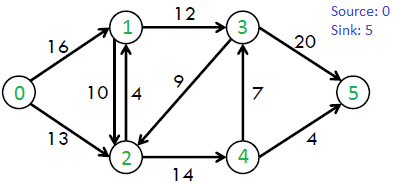
\includegraphics{ford_fulkerson11.png}
	}
	\only<2>{
	}
	\end{textarea}
}
\content
	{s2-400}
	{4}
	{400}{
	\begin{textarea}[]
	\only<1>{
		Consider a set of mobile computing clients in a certain town who each need to be connected to one of several possible “base stations”. We’ll suppose there are n clients, with the position of each client specified by its (x, y) coordinates in the plane. There are also m base stations, each of whose position is specified by (x, y) coordinates as well. 

We wish to connect each client to exactly one base station. Our choice of connections is constrained in the following ways: 
• There is a “range parameter” r. A client can only be connected to a base station that is within distance r of that client. 
• There is also a “load parameter” L. For any given base station, no more than L clients can be connected to it.

How would you represent this problem as a flow network? 
	}
	\only<2>{
		Let arr[0..n-1] be the input array and L(i) be the length of the LIS ending at index i such that arr[i] is the last element of the LIS :

L(i) = 1 + max( L(j) ) where 0 < j < i and arr[j] < arr[i]; or \newline
L(i) = 1, if no such j exists.
	}
	\end{textarea}
}
\content
	{s2-500}
	{5}
	{500}{
	\begin{textarea}[]
	\only<1>{
		Outline an algorithm for finding bottleneck edges (where increasing the capacity of this edge would increase the max) given the residual network. 
	}
	\only<2>{
		$c(i, j) = min_{i<k<j} {c(i, k) + c(k, j) + (dj − di)}$ 
where $c(i, j)$ is the min cost of cutting a log with left endpoint i and right endpoint j at all its marked locations. Start with $c(i, i+1)$ (consecutive cuts) and move outwards to $c(i, i+2), c(i, i+3)$ until the maximal distance $c(1, n)$, which gives the optimal score for the whole wood. Remember pointers to k that gave max score at each step, and trace back pointers to construct optimal solution. Each iteration
takes $O(n)$ (linear search between i and j) and there are $O(n^2)$ entries to fill. (a triangle, not really a square). from \url{https://courses.csail.mit.edu/6.006/fall11/rec/rec24.pdf}
	}
	\end{textarea}
}


% Greedy
\content                       % 4 arguments
	{s3-100}                     % question internal identifier
	{1}                          % subject number
	{100}{                       % question prize
        \begin{textarea}[]         % question/answer content
        \only<1>{                  % answer content
        	What does Djikstra’s algorithm find? Describe the algorithm. 
	}
        \only<2>{                  % question content
	}
        \end{textarea}
}

\content
	{s3-200}
	{2}
	{200}{
	\begin{textarea}[]
	\only<1>{
		How can you find MST using max heap?
	}
	\only<2>{
		By deleting all safe edges until MST is found.
	}
	\end{textarea}
}
\content
	{s3-300}
	{3}
	{300}{
	\begin{textarea}[]
	\only<1>{
		Not just any greedy approach to the activity-selection problem produces a maximum-size set of mutually compatible activities. Give an example to show that the approach of selecting the activity of least duration from among those that are compatible with previously selected activities does not work.
	}
	\only<2>{
	}
	\end{textarea}
}
\content
	{s3-400}
	{4}
	{400}{
	\begin{textarea}[]
	\only<1>{
		Graph Coloring Problem. Create a greedy algorithm. Is it optimal? What are it's bounds (num of colors)?
	}
	\only<2>{
		No. Max vertex degree +1.
	}
	\end{textarea}
}
\content
	{s3-500}
	{5}
	{500}{
	\begin{textarea}[]
	\only<1>{
		If negative edges are only adjacent to the source, can Dijkstra's algorithm produce a correct shortest path tree?
	}
	\only<2>{
		Yes.
	}
	\end{textarea}
}

% Approximation
\content                       % 4 arguments
	{s4-100}                     % question internal identifier
	{1}                          % subject number
	{100}{                       % question prize
        \begin{textarea}[]         % question/answer content
        \only<1>{                  % answer content
		Define approximation ratio.
	}
        \only<2>{                  % question content
	}
        \end{textarea}
}

\content
	{s4-200}
	{2}
	{200}{
	\begin{textarea}[]
	\only<1>{
		Give an example of a graph for which APPROX-VERTEX-COVER always yields a
suboptimal solution.
	}
	\only<2>{
	}
	\end{textarea}
}
\content
	{s4-300}
	{3}
	{300}{
	\begin{textarea}[]
	\only<1>{
		Consider each of the following words as a set of letters: farid; dash; drain;
heard; lost; nose; shun; slate; snare; threadg. Show which set cover GREEDY-SET-COVER produces when we break ties in favor of the word that appears first in the dictionary.
	}
	\only<2>{
	}
	\end{textarea}
}
\content
	{s4-400}
	{4}
	{400}{
	\begin{textarea}[]
	\only<1>{
		GREEDY-SET-COVER can return a number of different solutions, depending on how we break ties when picking a set Give a procedure BAD-SET-COVER-INSTANCE(n) that returns an n-element instance of the set-covering problem for which, depending on how we break ties while picking a set, GREEDY-SET-COVER can return a number of different solutions that is exponential in n.
	}
	\only<2>{
	}
	\end{textarea}
}
\content
	{s4-500}
	{5}
	{500}{
	\begin{textarea}[]
	\only<1>{
		For the travelling salesman problem, proof that the following algorithm produces a 2-approximation:
APPROX-TSP-TOUR (G)
Select a vertex r 2 G:V to be a “root” vertex
Compute a minimum spanning tree T for G from root r using MST-PRIM (G, r)
Let H be a list of vertices, ordered according to when they are first visited
in a preorder tree walk of T
Return the hamiltonian cycle H
	}
	\only<2>{
		A full walk of T lists the vertices when they are first visited and also whenever they are returned to after a visit to a subtree. Since the full walk traverses every edge of T exactly twice, we have $c(W) =  2*c(T) \rightarrow c(W) \leq 2*c(H^*)$. Unfortunately, the full walk W is generally not a tour, since it visits some vertices more than once. By the triangle inequality, however, we can delete a visit to any vertex from W and the cost does not increase.
	}
	\end{textarea}
}

\end{document}
